\documentclass[useAMS]{biom}\usepackage[]{graphicx}\usepackage[]{color}
%% maxwidth is the original width if it is less than linewidth
%% otherwise use linewidth (to make sure the graphics do not exceed the margin)
\makeatletter
\def\maxwidth{ %
  \ifdim\Gin@nat@width>\linewidth
    \linewidth
  \else
    \Gin@nat@width
  \fi
}
\makeatother

\definecolor{fgcolor}{rgb}{0.345, 0.345, 0.345}
\newcommand{\hlnum}[1]{\textcolor[rgb]{0.686,0.059,0.569}{#1}}%
\newcommand{\hlstr}[1]{\textcolor[rgb]{0.192,0.494,0.8}{#1}}%
\newcommand{\hlcom}[1]{\textcolor[rgb]{0.678,0.584,0.686}{\textit{#1}}}%
\newcommand{\hlopt}[1]{\textcolor[rgb]{0,0,0}{#1}}%
\newcommand{\hlstd}[1]{\textcolor[rgb]{0.345,0.345,0.345}{#1}}%
\newcommand{\hlkwa}[1]{\textcolor[rgb]{0.161,0.373,0.58}{\textbf{#1}}}%
\newcommand{\hlkwb}[1]{\textcolor[rgb]{0.69,0.353,0.396}{#1}}%
\newcommand{\hlkwc}[1]{\textcolor[rgb]{0.333,0.667,0.333}{#1}}%
\newcommand{\hlkwd}[1]{\textcolor[rgb]{0.737,0.353,0.396}{\textbf{#1}}}%

\usepackage{framed}
\makeatletter
\newenvironment{kframe}{%
 \def\at@end@of@kframe{}%
 \ifinner\ifhmode%
  \def\at@end@of@kframe{\end{minipage}}%
  \begin{minipage}{\columnwidth}%
 \fi\fi%
 \def\FrameCommand##1{\hskip\@totalleftmargin \hskip-\fboxsep
 \colorbox{shadecolor}{##1}\hskip-\fboxsep
     % There is no \\@totalrightmargin, so:
     \hskip-\linewidth \hskip-\@totalleftmargin \hskip\columnwidth}%
 \MakeFramed {\advance\hsize-\width
   \@totalleftmargin\z@ \linewidth\hsize
   \@setminipage}}%
 {\par\unskip\endMakeFramed%
 \at@end@of@kframe}
\makeatother

\definecolor{shadecolor}{rgb}{.97, .97, .97}
\definecolor{messagecolor}{rgb}{0, 0, 0}
\definecolor{warningcolor}{rgb}{1, 0, 1}
\definecolor{errorcolor}{rgb}{1, 0, 0}
\newenvironment{knitrout}{}{} % an empty environment to be redefined in TeX

\usepackage{alltt}

%  If your system does not have the AMS fonts version 2.0 installed, then
%  remove the useAMS option.
%
%  useAMS allows you to obtain upright Greek characters.
%  e.g. \umu, \upi etc.  See the section on "Upright Greek characters" in
%  this guide for further information.
%
%  If you are using AMS 2.0 fonts, bold math letters/symbols are available
%  at a larger range of sizes for NFSS release 1 and 2 (using \boldmath or
%  preferably \bmath).
% 
%  Other options are described in the user guide. Here are a few:
% 
%  -  If you use Patrick Daly's natbib  to cross-reference your 
%     bibliography entries, use the usenatbib option
%
%  -  If you use \includegraphics (graphicx package) for importing graphics
%     into your figures, use the usegraphicx option
% 
%  If you wish to typeset the paper in Times font (if you do not have the
%  PostScript Type 1 Computer Modern fonts you will need to do this to get
%  smoother fonts in a PDF file) then uncomment the next line
%  \usepackage{Times}

%%%%% PLACE YOUR OWN MACROS HERE %%%%%

\def\bSig\mathbf{\Sigma}
\newcommand{\VS}{V\&S}
\newcommand{\tr}{\mbox{tr}}

%  The rotating package allows you to have tables displayed in landscape
%  mode.  The rotating package is NOT included in this distribution, but
%  can be obtained from the CTAN archive.  USE OF LANDSCAPE TABLES IS
%  STRONGLY DISCOURAGED -- create landscape tables only as a last resort if
%  you see no other way to display the information.  If you do do this,
%  then you need the following command.

%\usepackage[figuresright]{rotating}

%%%%%%%%%%%%%%%%%%%%%%%%%%%%%%%%%%%%%%%%%%%%%%%%%%%%%%%%%%%%%%%%%%%%%

%  Here, place your title and author information.  Note that in 
%  use of the \author command, you create your own footnotes.  Follow
%  the examples below in creating your author and affiliation information.
%  Also consult a recent issue of the journal for examples of formatting.

\title[This is an Example of Recto Running Head]{This is an Example of
an Article Title This is an Example of an Article Title}

%  Here are examples of different configurations of author/affiliation
%  displays.  According to the Biometrics style, in some instances,
%  the convention is to have superscript *, **, etc footnotes to indicate 
%  which of multiple email addresses belong to which author.  In this case,
%  use the \email{ } command to produce the emails in the display.

%  In other cases, such as a single author or two authors from 
%  different institutions, there should be no footnoting.  Here, use
%  the \emailx{ } command instead. 

%  The examples below corrspond to almost every possible configuration
%  of authors and may be used as a guide.  For other configurations, consult
%  a recent issue of the the journal.

%  Single author -- USE \emailx{ } here so that no asterisk footnoting
%  for the email address will be produced.

%\author{John Author\emailx{email@address.edu} \\
%Department of Statistics, University of Warwick, Coventry CV4 7AL, U.K.}

%  Two authors from the same institution, with both emails -- use
%  \email{ } here to produce the asterisk footnoting for each email address

%\author{John Author$^{*}$\email{author@address.edu} and
%Kathy Authoress$^{**}$\email{email2@address.edu} \\
%Department of Statistics, University of Warwick, Coventry CV4 7AL, U.K.}

%  Exactly two authors from different institutions, with both emails  
%  USE \emailx{ } here so that no asterisk footnoting for the email address
%  is produced.

\author
{John Author\emailx{author@address.edu} \\
Department of Statistics, University of Warwick, Coventry CV4 7AL, U.K. 
\and
Kathy Author\emailx{anotherauthor@address.edu} \\
Department of Biostatistics, University of North Carolina at Chapel Hill, 
Chapel Hill, North Carolina, U.S.A.}

%  Three or more authors from same institution with all emails displayed
%  and footnoted using asterisks -- use \email{ } 

%\author{John Author$^*$\email{author@address.edu}, 
%Jane Author$^{**}$\email{jane@address.edu}, and 
%Dick Author$^{***}$\email{dick@address.edu} \\
%Department of Statistics, University of Warwick, Coventry CV4 7AL, U.K}

%  Three or more authors from same institution with one corresponding email
%  displayed

%\author{John Author$^*$\email{author@address.edu}, 
%Jane Author, and Dick Author \\
%Department of Statistics, University of Warwick, Coventry CV4 7AL, U.K}

%  Three or more authors, with at least two different institutions,
%  more than one email displayed 

%\author{John Author$^{1,*}$\email{author@address.edu}, 
%Kathy Author$^{2,**}$\email{anotherauthor@address.edu}, and 
%Wilma Flinstone$^{3,***}$\email{wilma@bedrock.edu} \\
%$^{1}$Department of Statistics, University of Warwick, Coventry CV4 7AL, U.K \\
%$^{2}$Department of Biostatistics, University of North Carolina at 
%Chapel Hill, Chapel Hill, North Carolina, U.S.A. \\
%$^{3}$Department of Geology, University of Bedrock, Bedrock, Kansas, U.S.A.}

%  Three or more authors with at least two different institutions and only
%  one email displayed

%\author{John Author$^{1,*}$\email{author@address.edu}, 
%Wilma Flinstone$^{2}$, and Barney Rubble$^{2}$ \\
%$^{1}$Department of Statistics, University of Warwick, Coventry CV4 7AL, U.K \\
%$^{2}$Department of Geology, University of Bedrock, Bedrock, Kansas, U.S.A.}
\IfFileExists{upquote.sty}{\usepackage{upquote}}{}


\begin{document}

%  This will produce the submission and review information that appears
%  right after the reference section.  Of course, it will be unknown when
%  you submit your paper, so you can either leave this out or put in 
%  sample dates (these will have no effect on the fate of your paper in the
%  review process!)

\date{{\it Received October} 2007. {\it Revised February} 2008.  {\it
Accepted March} 2008.}

%  These options will count the number of pages and provide volume
%  and date information in the upper left hand corner of the top of the 
%  first page as in published papers.  The \pagerange command will only
%  work if you place the command \label{firstpage} near the beginning
%  of the document and \label{lastpage} at the end of the document, as we
%  have done in this template.

%  Again, putting a volume number and date is for your own amusement and
%  has no bearing on what actually happens to your paper!  

\pagerange{\pageref{firstpage}--\pageref{lastpage}} 
\volume{64}
\pubyear{2008}
\artmonth{December}

%  The \doi command is where the DOI for your paper would be placed should it
%  be published.  Again, if you make one up and stick it here, it means 
%  nothing!

\doi{10.1111/j.1541-0420.2005.00454.x}

%  This label and the label ``lastpage'' are used by the \pagerange
%  command above to give the page range for the article.  You may have 
%  to process the document twice to get this to match up with what you 
%  expect.  When using the referee option, this will not count the pages
%  with tables and figures.  

\label{firstpage}

%  put the summary for your paper here

\begin{abstract}
This is the summary for this paper.
\end{abstract}

%  Please place your key words in alphabetical order, separated
%  by semicolons, with the first letter of the first word capitalized,
%  and a period at the end of the list.
%

\begin{keywords}
A key word; But another key word; Still another key word; Yet another key word.
\end{keywords}

%  As usual, the \maketitle command creates the title and author/affiliations
%  display 

\maketitle

%  If you are using the referee option, a new page, numbered page 1, will
%  start after the summary and keywords.  The page numbers thus count the
%  number of pages of your manuscript in the preferred submission style.
%  Remember, ``Normally, regular papers exceeding 25 pages and Reader Reaction 
%  papers exceeding 12 pages in (the preferred style) will be returned to 
%  the authors without review. The page limit includes acknowledgements, 
%  references, and appendices, but not tables and figures. The page count does 
%  not include the title page and abstract. A maximum of six (6) tables or 
%  figures combined is often required.''

%  You may now place the substance of your manuscript here.  Please use
%  the \section, \subsection, etc commands as described in the user guide.
%  Please use \label and \ref commands to cross-reference sections, equations,
%  tables, figures, etc.
%
%  Please DO NOT attempt to reformat the style of equation numbering!
%  For that matter, please do not attempt to redefine anything!

\section{Introduction}
\label{s:intro}

Here is the introduction. The file \texttt{biomsample.tex} gives an
example of using the \texttt{natbib} package to cross-reference
citations from the bibliography.  Here, we just do this manually to
demonstrate that the old-fashioned way also is acceptable.  See the
comment right before the bibliography section below for information on
using BiBTeX.

Please note that, although this document class produces a final
product that is very close to the format and appearance of a typeset
\textit{Biometrics} article, there may be some idiosyncracies that
cause the format to deviate slightly from that in the journal.  These
will be corrected at the typesetting phase should your paper be accepted
and forwarded for publication.  So do not worry if such things occur!

\begin{knitrout}
\definecolor{shadecolor}{rgb}{0.969, 0.969, 0.969}\color{fgcolor}\begin{kframe}
\begin{alltt}
\hlkwd{plot}\hlstd{(cars)}
\end{alltt}
\end{kframe}
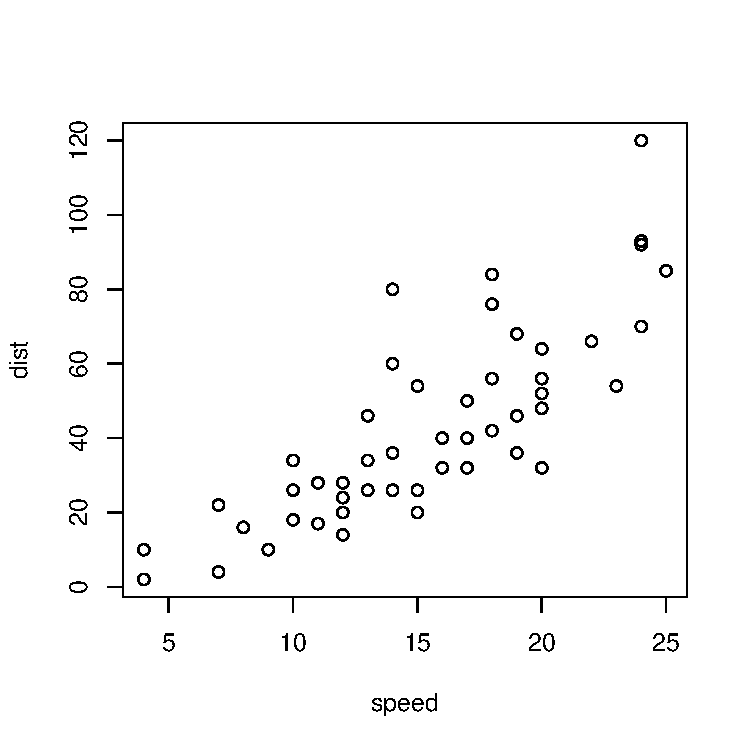
\includegraphics[width=\maxwidth]{figure/cars} 

\end{knitrout}


\section{Model}
\label{s:model}

\subsection{First Model Subsection}

The Cox model (Cox, 1972) is one of the most widely used statistical
models.  Hastie, Tibshirani, and Friedman (2001) is an example of a
citation to a work with three authors.  The first time you reference
one of these in the text, use all the authors names. However, in all
subsequent references, just use Hastie et al. (2001).  Works with four
or more authors are always referenced in the text using ``et al.''
All authors names should appear in the bibliography for all entries.

\subsection{Second Model Subsection}

Please use a recent issue of \textit{Biometrics} as a guide to the style
for citations and bibliography entries, and follow that style exactly!!


\section{Inference}
\label{s:inf}

Please see the file \texttt{biomsample.tex} for fancy examples of making
tables.  Here is a very simple one.  Use \texttt{table} for tables
that are narrow enough to fit in one column of the typeset journl; use
\texttt{table*} for tables that need to span two columns.  For
figures, use of \texttt{figure} and \texttt{figure*} is analogous. 

\begin{table}
\caption{This is a simple table.}
\label{t:one}
\begin{center}
\begin{tabular}{lrrr}
\Hline
Estimator & \multicolumn{1}{c}{$\beta_1$} &  \multicolumn{1}{c}{$\beta_2$} & 
\multicolumn{1}{c}{$\beta_3$} \\ \hline
MLE & 10.18 & $-$3.26 & 0.13 \\
OLS & 9.92 & $-$3.19 & 0.11 \\
WLS & 9.88 & $-$3.33 & 0.12 \\
\hline
\end{tabular}
\end{center}
\end{table}

You can experiment with fancier tables than Table~\ref{t:one}.

We can get bold symbols using \verb+\bmath+, for example, $\bmath{\alpha}_i$.

\section{Discussion}
\label{s:discuss}

Put your final comments here. 

%  The \backmatter command formats the subsequent headings so that they
%  are in the journal style.  Please keep this command in your document
%  in this position, right after the final section of the main part of 
%  the paper and right before the Acknowledgements, Supplementary Materials,
%  and References sections. 

\backmatter

%  This section is optional.  Here is where you will want to cite
%  grants, people who helped with the paper, etc.  But keep it short!

\section*{Acknowledgements}

The authors thank Professor A. Sen for some helpful suggestions,
Dr C. R. Rangarajan for a critical reading of the original version of the
paper, and an anonymous referee for very useful comments that improved
the presentation of the paper.\vspace*{-8pt}

%  If your paper refers to supplementary web material, then you MUST
%  include this section!!  See Instructions for Authors at the journal
%  website http://www.biometrics.tibs.org

\section*{Supplementary Materials}

Web Appendix A, referenced in Section~\ref{s:model}, is available with
this paper at the Biometrics website on Wiley Online
Library.\vspace*{-8pt}

%  Here, we create the bibliographic entries manually, following the
%  journal style.  If you use this method or use natbib, PLEASE PAY
%  CAREFUL ATTENTION TO THE BIBLIOGRAPHIC STYLE IN A RECENT ISSUE OF
%  THE JOURNAL AND FOLLOW IT!  Failure to follow stylistic conventions
%  just lengthens the time spend copyediting your paper and hence its
%  position in the publication queue should it be accepted.

%  We greatly prefer that you incorporate the references for your
%  article into the body of the article as we have done here 
%  (you can use natbib or not as you choose) than use BiBTeX,
%  so that your article is self-contained in one file.
%  If you do use BiBTeX, please use the .bst file that comes with 
%  the distribution.

\begin{thebibliography}{}

\bibitem{ } Cox, D. R. (1972). Regression models and life tables (with
discussion).  \textit{Journal of the Royal Statistical Society, Series B}
\textbf{34,} 187--200.

\bibitem{ }  Hastie, T., Tibshirani, R., and Friedman, J. (2001). \textit{The 
Elements of Statistical Learning: Data Mining, Inference, and Prediction}.
New York: Springer.

\end{thebibliography}

\appendix

%  To get the journal style of heading for an appendix, mimic the following.

\section{}
\subsection{Title of appendix}

Put your short appendix here.  Remember, longer appendices are
possible when presented as Supplementary Web Material.  Please 
review and follow the journal policy for this material, available
under Instructions for Authors at \texttt{http://www.biometrics.tibs.org}.

\label{lastpage}

\end{document}
